\documentclass[10pt]{standalone}
\usepackage{pgfplots}
\pgfplotsset{compat=1.15}
\usepackage{mathrsfs}
\usetikzlibrary{arrows}
\pagestyle{empty}
\begin{document}

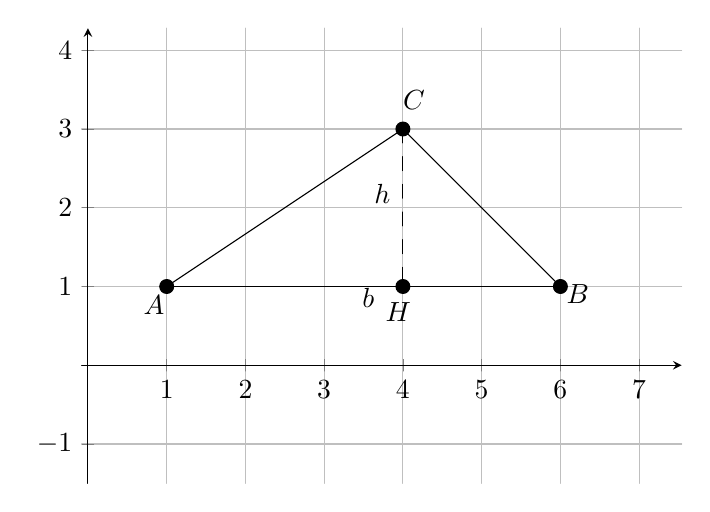
\begin{tikzpicture}[line cap=round,line join=round,>=triangle 45,x=1.0cm,y=1.0cm]
\begin{axis}[
x=1.0cm,y=1.0cm,
axis lines=middle,
ymajorgrids=true,
xmajorgrids=true,
xmin=-0.0799999999999999,
xmax=7.5399999999999965,
ymin=-1.500000000000001,
ymax=4.280000000000001,
xtick={-0.0,1.0,...,7.0},
ytick={-1.0,0.0,...,4.0},]
\clip(-0.08,-1.5) rectangle (7.54,4.28);
\draw (1.,1.)-- (6.,1.);
\draw (6.,1.)-- (4.,3.);
\draw (4.,3.)-- (1.,1.);
\draw [dash pattern=on 5pt off 5pt] (4.,3.)-- (4.,1.);
\begin{scriptsize}
\draw [fill=black] (1.,1.) circle (2.5pt);
\draw[color=black] (0.84,0.77) node {$A$};
\draw [fill=black] (6.,1.) circle (2.5pt);
\draw[color=black] (6.22,0.91) node {$B$};
\draw [fill=black] (4.,3.) circle (2.5pt);
\draw[color=black] (4.14,3.37) node {$C$};
\draw[color=black] (3.56,0.85) node {$b$};
\draw [fill=black] (4.,1.) circle (2.5pt);
\draw[color=black] (3.94,0.67) node {$H$};
\draw[color=black] (3.74,2.17) node {$h$};
\end{scriptsize}
\end{axis}
\end{tikzpicture}
\end{document}